Firebase ist eine Backend-as-a-Service (BaaS) Plattform von Google für mobile oder Web-Anwendungen. 
Sie soll es dem Entwickler ermöglichen, einfacher und effizienter Funktionen auf verschiedenen Plattformen bereitzustellen stellt Tools und Infrastruktur zur Verfügung.
Mit dem Firebase SDK bietet die Plattform API Schnittstellen zu den jeweiligen Tools, welche direkt in die Anwendung integriert werden können, ohne dass serverseitiger Code dafür notwendig ist.
Die Firebase Inc. wurde 2011 von James Tamplin und Andrew Lee gegründet und letztendlich 2014 von Google übernommen.\footnote{\href{https://firebase.googleblog.com/2014/10/firebase-is-joining-google.html}{firebase.googleblog.com}, zuletzt aufgerufen am 03.05.2021}
Teile der SDK stehen seit der Google I/O 2017 unter der Apache 2.0 Lizenz, sind somit also Open-Source.\footnote{\href{https://opensource.googleblog.com/2017/05/open-sourcing-firebase-sdks.html}{opensource.googleblog.com}, zuletzt aufgerufen am 03.05.2021}\\
\\
Es existieren zwei Kostenmodelle für die Nutzung von Firebase: Ein kostenloses Modell \glqq Spark Plan\grqq und ein pay-as-you-go \glqq Blaze Plan\grqq . Das kostenlosen Modell beinhaltet die wichtigsten Tools, viele dieser Tools sind jedoch begrenzt durch beispielsweise Bandbreite oder Speicherplatz.
Der Pay-as-you-go Plan ist eine Erweiterung des kostenlosen Plans. 
Er bietet daher das Nutzen von Tools bis zu einem gewissen Limit kostenfrei an; darüber hinaus kostet es jedoch dann pro Nutzung.\\
\\
Ein Firebase Projekt ist die oberste Ebene in Firebase. 
Ein Projekt ist letztendlich ein \textit{Google Cloud Projekt}, welches mit speziellen Konfigurationsmöglichkeiten und Services ausgestattet ist. 
Es beinhaltet die Verknüpfung zu den einzelnen Anwendungen (also bspw. Android-, iOS- oder Webanwendung). Nun können variabel Tools, sog. Firebase products hinzugefügt werden. Diese Produkte lassen sich grundlegend in drei Kategorien einteilen. Die hier relevantesten werden im Folgenden besprochen.\cite{firebase2021}

\subsubsection{Firebase Authentifizierung}
Die Authentifizierung gehört zu den \glqq Build\grqq Produkten und bietet eine Token-basierte Nutzerauthentifizierung. 
Hierbei kann zwischen verschiedenen Anmeldeoptionen gewählt werden: klassisch mit E-Mail und Passwort, mit OAuth2.0 Integration für Social Media (Google, Facebook, Twitter, Github, ...) oder per Telefonnummer.
Jeder Nutzer erhält eine einzigartige ID und ein zugehöriges Nutzerobjekt in einer NoSQL Datenbank. Grundlegende Werte wie E-Mail Adresse oder Name können hier abgespeichert werden; zusätzliche Informationen müssen über einen weiteren Datenbank Service abgespeichert werden.
Für die Verwaltung eines Accounts bietet dieses Tool auch eingebaute E-Mail Aktionen an - bspw. Passwort zurücksetzen oder E-Mail Adresse bestätigen.\\
\\
Ein Firebase Nutzer Objekt repräsentiert den Account eines Nutzers, welcher sich von einer Anwendung aus beim zentralen Firebase Projekt angemeldet hat.
Die Instanz eines Firebase Nutzers ist somit unabhängig von der Authentifizierungsinstanz der Anwendung, also kann eine Anwendung mehrere Nutzer anmelden, jedoch kann sich auch ein Nutzer auf mehreren Anwendungen anmelden.
Ist ein Nutzer authentifiziert, erhält die Anwendung eine Referenz des Nutzers, welche so lange existiert, bis er wieder abgemeldet ist.\cite{firebase2021}

\subsubsection{Cloud Firestore}
\label{sec:firestore}
Als Datenbank Lösung bietet Firebase zwei unterschiedliche Produkte an: Cloud Firestore und Realtime Database.
Firestore ist hier neuer, jedoch ersetzt es Realtime Database nicht. \\
Cloud Firestore ist eine flexible und auf Skalierung ausgesetzte NoSQL Cloud Datenbank, welche unter anderem die Echtzeitsynchronisierung der Daten zwischen Anwendung und Server ermöglicht.
Zusätzlich zu REST und RPC APIs in iOS, Android und web SDKs ist Firestore auch in nativen Node.js, Java, Python und Go SDKs verfügbar.\\
\\

\begin{wrapfigure}{R}{0.4\textwidth}
	\begin{center}
		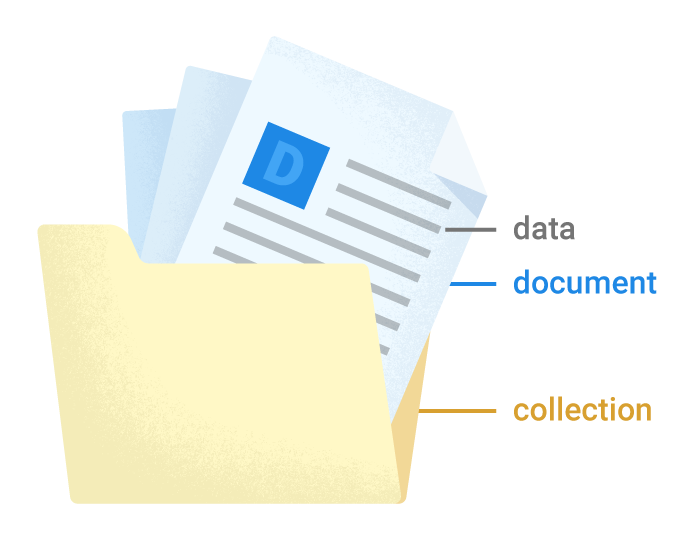
\includegraphics[width=0.35\textwidth]{./Theoretische_Grundlagen/images/firestore_datastucture.png}
	\end{center}
	\caption{Datenmodell in Firebase \protect \footnotemark}
	\label{fig:firestore_data_structure}
\end{wrapfigure}
\footnotetext{Quelle: \cite{firebase2021}}

Das Datenmodell ist hierarchisch aufgebaut, wobei Daten in Dokumenten (documents) und Dokumente in Sammlungen (collections) gespeichert sind. 
Mithilfe von Sammlungen werden die Daten voneinander abgetrennt und hierüber können Abfragen erstellt werden.
Grundlegende Datentypen sind String, Integer und Boolean, jedoch können auch komplexe Datentypen wie Maps, Arrays oder Geopoints. Unter-Sammlungen und darin verstaute Dokumente sind ebenfalls möglich.\\
\\
Abfragen werden auf Dokumentenebene erstellt, damit nicht eine gesamte Sammlung aufgerufen werden muss.
Dies kann über direkte Sortierung, Filter und/oder Limitierung bzw. genaue Auswahl eines Dokumentes bewerkstelligt werden.
Bei einer Abfrage erhält man einen \textit{Data Snapshot}, wodurch über Änderungen in Echtzeit informiert und diese angezeigt werden können.
Damit es jedoch zu keinen fehlerhaften Daten führt, gelten hier atomare Eigenschaften für Transaktionen.
Eine Transaktion ist eine Folge von Datenbankanweisungen, welche entweder alle gemeinsam oder gar nicht ausgeführt werden. 
Eine Transaktion ist nur dann erfolgreich, wenn alle Anweisungen auf eine Datenbank vollständig geschlossen sind. 
Ist dies nicht der Fall, werden alle Anweisungen bis zum Stand vor der Transaktion rückgängig gemacht. Das nennt man Rollback.\\
\\
Die Sicherheit der Daten stellt Cloud Firestore für Mobil- und Webclient-Bibliotheken über die Firestore-Sicherheitsregeln her. Diese bieten sowohl Zugriffsverwaltung und -authentifizierung, jedoch könne auch Daten hiermit für die Konsistenz der Datenbank validiert werden. 
\medskip
\begin{lstlisting}[caption=Beschränkung des Zugriffs auf Dokumente der Sammlung \texttt{cities}, label=lst:firestorerules_basic]
	service cloud.firestore {
		match /databases/{database}/documents {
			match /cities/{city} {
				allow read, write: if request.auth != null;
			}
		}
	}
\end{lstlisting}
\medskip
Im Beispiel \ref{lst:firestorerules_basic} wird der Lese- und Schreibzugriff auf ein Dokument der Sammlung \texttt{cities} beschränkt. 
Nur falls der anfragende Nutzer eine valide Authentifizierung besitzt, erhält er Zugriff auf das angefragte Dokument. 
Diese simple Darstellung ist jedoch für den wirklichen Produktionseinsatz mit Vorsicht zu nutzen. 
Oftmals müssen \texttt{read} und \texttt{write} in detailliertere Vorgänge aufgeteilt werden. Ein \texttt{read} wird spezialisiert in \texttt{get} und \texttt{list}, wobei ein \texttt{write} in \texttt{create}, \texttt{update} und \texttt{delete} unterteilt werden kann.
Ein \texttt{list} ermöglicht es hierbei auf Sammlungen, also die einzelnen Dokumenten IDs lesend zuzugreifen, jedoch nicht auf die Daten einzelner Dokumente. Hierfür wird dann ein \texttt{get} benötigt. 
Mittels \texttt{create} erhält man Schreibzugriff auf nicht existierende Dokumente, durch \texttt{update} auf bereits vorhandene und Löschrechte ganzer Dokumente erhält man über den \texttt{delete} Operator.\\
\\
Sicherheitsregeln werden gleich dem Datenmodell hierarchisch aufgebaut und ermöglichen differenzierte Zugriffsbeschränkungen auf jeder Ebene.
In Codebeispiel \ref{lst:firestorerules_hierarchy} beinhaltet jedes Dokument (Stadt) der Sammlung \texttt{cities} eine Unter-Sammlung \texttt{landmarks}. Nun lässt sich der Zugriff auf beide separat regeln.
Bei der Sammlung \texttt{villages} hingegen wurde der rekursive Platzhalter verwendet. Hiermit sind Zugriffsregeln auf allen tieferen Ebenen gleich.
Beim Verschachteln von \texttt{match} ist der innere Pfad immer relativ zum äußeren.

Wichtig zu wissen ist hierzu noch, dass falls mehrere \texttt{allow} Ausdrücke auf eine Anfrage zutreffen, wird der Zugriff erlaubt sobald \textbf{eine} Bedingung wahr, also erfüllt ist.

\medskip
\begin{lstlisting}[caption=Hierarchische Zugriffsbeschränkung, label=lst:firestorerules_hierarchy]
	service cloud.firestore {
		match /databases/{database}/documents {
			match /cities/{city} {
				allow read, write: if <condition>;
				
				// Explicitly define rules for the 'landmarks' subcollection
				match /landmarks/{landmark} {
					allow read, write: if <condition>;
				}
			}
			match /villages/{document=**} {
				allow read, write: if <condition>;
			}
		}
	}
\end{lstlisting}
\medskip

Wie bereits oben besprochen können diese Regeln auch zur Validierung von Daten genutzt werden, damit die atomare Eigenschaft von Transaktionen bestehen bleibt.
Hierzu kann die \texttt{getAfter()} Funktion genutzt werden. 
Mit dieser kann man auf Zustand eines Dokumentes zugreifen und diesen validieren, nachdem einer Folge von Anweisungen ausgeführt, jedoch diese noch nicht auf der Firestore Datenbank abgeschlossen wurde.
Im Beispiel \ref{lst:firestorerules_validation} existieren zwei Sammlungen: \texttt{cities} und \texttt{countries}. 
Jedes \texttt{country} Dokument beinhaltet das Feld \texttt{last\_updated} um zu wissen, welche Stadt innerhalb eines Landes zuletzt aktualisiert wurde.
Hierzu wird in den Sicherheitsregeln nach jedem Schreibzugriff auf ein \texttt{city} Dokument gleichzeitig auch das Feld des zugehörigen Landes aktualisiert.\cite{firebase2021}
\medskip
\begin{lstlisting}[caption=Datenvalidierung für atomare Operationen, label=lst:firestorerules_validation]
	service cloud.firestore {
		match /databases/{database}/documents {
			// If you update a city doc, you must also
			// update the related country's last_updated field.
			match /cities/{city} {
				allow write: if request.auth != null &&
				getAfter(
				/databases/$(database)/documents/countries/$(request.resource.data.country)
				).data.last_updated == request.time;
			}
			
			match /countries/{country} {
				allow write: if request.auth != null;
			}
		}
	}
\end{lstlisting}
\medskip

\subsubsection{Cloud Storage}
Um Filme, Videos oder andere Nutzer-generierte Inhalte abspeichern zu können, bietet Firebase Cloud Storage an. 
Durch das Firebase SDK für Cloud Storage können Dateien direkt von Client-Anwendungen hoch- bzw. heruntergeladen werden.
Aufgrund von möglicher schlechter Verbindung kann mithilfe von robusten Operationen der Prozess des Hoch- bzw. Herunterladens bei besserer Verbindung an der Stelle weiter geladen werden, an welcher dieser unterbrochen wurde.
Ähnlich wie bei Cloud Firestore in Kapitel \ref{sec:firestore} bestimmen auch hier Sicherheitsregeln den Zugriff auf bestimmte Dokumente.\\
Zusätzlich hierzu sind weitere Metadaten verfügbar: \texttt{contentType} und \texttt{size}. 
Mit ihnen lassen sich die Dateien beispielsweise validieren.
Im Code \ref{lst:storagerules_validation} können Dateien nur hochgeladen werden, falls sie eine Größe kleiner 5 MB besitzen.
\medskip
\begin{lstlisting}[caption=Validierung nach Dateigröße, label=lst:storagerules_validation]
	service firebase.storage {
		match /b/{bucket}/o {
			match /images/{imageId} {
				allow write: if request.resource.size < 5 * 1024 * 1024
				&& request.resource.contentType.matches('image/.*');
			}
		}
		
\end{lstlisting}
\medskip
Außerdem lassen sich durch Cloud Functions aus dem nächsten Kapitel Prozesse automatisieren. Beispielsweise lässt sich beim Upload eines Bildes direkt ein individuelles Thumbnail erstellen lassen.\cite{firebase2021}
\subsubsection{Cloud Functions}
\label{sec:cloudfunctions}
Da Firebase - bis auf vereinfachte Sicherheitsregeln - eigentlich keinen Backend Code benötigt, jedoch manche Features eben genau diesen brauchen, um beispielsweise Benachrichtigungen an Nutzer zu senden oder Bilder zu komprimieren, existieren Cloud Functions.\\
Diese ermöglichen es, als Antwort auf ein Event automatisch oder durch HTTPS Anfrage manuell Backend Code auszuführen.
Der gesamte Code ist hierbei in der Google Cloud gespeichert und wird in einer verwalteten Umgebung ausgeführt.
Als Programmiersprache kann sowohl JavaScript als auch Typescript verwendet werden.\\
\\
\glqq Google Cloud Functions ist die serverlose Computerlösung von Google zum erStellen ereignisgesteuerter Anwendungen.\grqq \cite{firebase2021} 
Es kann sowohl auf der Google Cloud Platform (GCP) also auch für Firebase genutzt werden. 
Es ist bei beiden ein Verbindungsglied zwischen Logik und entsprechenden Diensten, welche dadurch mit serverseitigen Code erweitert und kombiniert werden.
\begin{figure}[htb]
	\begin{center}
		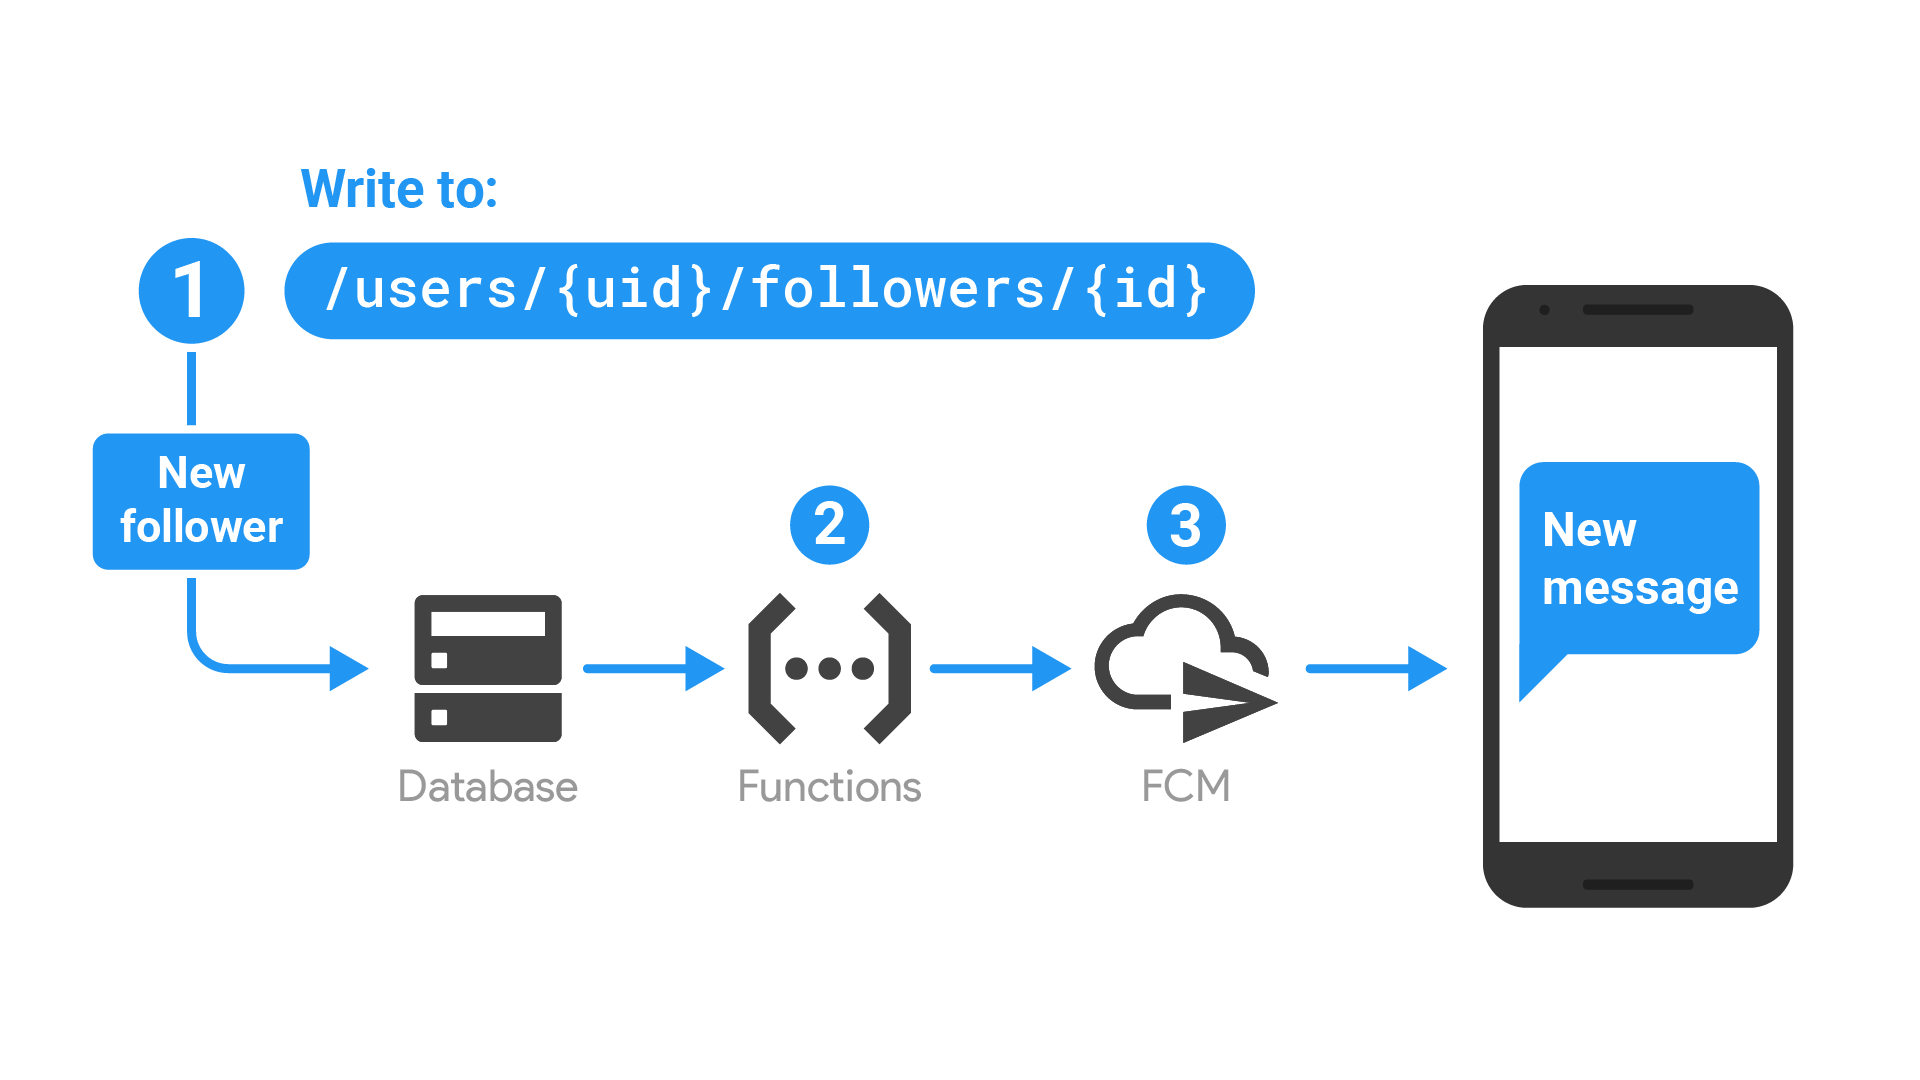
\includegraphics[scale=0.2]{Theoretische_Grundlagen/images/firebase_functions_notify.png}
	\end{center}
	\caption{Cloud Functions Anwendungsfall Benachrichtigung}
	\label{fig:functions_notifications}
\end{figure}
In Abbildung \ref{fig:functions_notifications} ist ein typischer Anwendungsfall beschrieben. 
Ein Event auf der Datenbank wird ausgelöst, hier ein neuer Nutzer folgt einem weiteren Nutzer.
Es wird also ein Dokument in der Unter-Sammlung \texttt{followers} erzeugt. Diese Unter-Sammlung befindet sich innerhalb des Dokumentes \texttt{uid} der Sammlung \texttt{users}.
Im zweiten Schritt erstellt die Funktion eine Nachricht, welche über Firebase Cloud Messaging (FCM) versendet werden soll.
Über abgespeicherte Tokens sendet FCM die Benachrichtigung an das Gerät des Nuters \texttt{uid}.\cite{firebase2021}
\subsubsection{Cloud Messaging}
Firebase Cloud Messaging ist eine plattformübergreifende Messaging-Lösung zum zuverlässigen Versenden von Nachrichten an Nutzergeräte.
In Abbildung \ref{fig:cloudmessaging_architecture} ist die Architektur dieses Tools dargestellt.
Hierbei wird es grundlegend in das Erstellen, Transportieren und Empfangen der Nachrichten unterteilt.\cite{firebase2021}\\
\begin{itemize}
	\item \textbf{Erstellen} Die zu versendenden Nachrichten können, wie in Kapitel \ref{sec:cloudfunctions} beschrieben, manuell oder automatisiert erzeugt werden. 
	Bei der Automatisierung ist wichtig, dass die Nachrichten in einer vertrauenswürdigen Serverumgebung erstellt werden, damit alle Nachrichtentypen unterstützt werden (Schritt 1). 
	Das FCM Backend akzeptiert dann in Schritt 2 Nachrichtenanfragen, ordnet die Nachrichten verschiedenen Themen zu und erzeugt unter anderem Metadaten für Nachrichten, wie bspw. die Nachricht ID. 
	\item \textbf{Transportieren} Die Nachrichten werden hierbei an die entsprechenden Geräte weitergeleitet.
	Da verschiedene Geräte auf unterschiedlichen Plattformen basieren, muss die Transportschicht auf Plattformebene arbeiten.
	Hierfür werden folgende Ebenen genutzt:
	\begin{itemize}
		\item Android Transport Layer (ATL) für Android-Geräte mit Google Play-Diensten
		\item Apple Push Notification Service (APNs) für iOS-Geräte
		\item Web-Push-Protokoll für Web-Apps
	\end{itemize}
	\item \textbf{Empfangen} Das FCM SDK behandelt die Benachrichtigung oder Nachricht. Dies ist abhängig vom Vorder-/ Hintergrundstatus der Anwendung und der jeweiligen Anwendungslogik.
\end{itemize}


\begin{figure}[htb]
	\begin{center}
		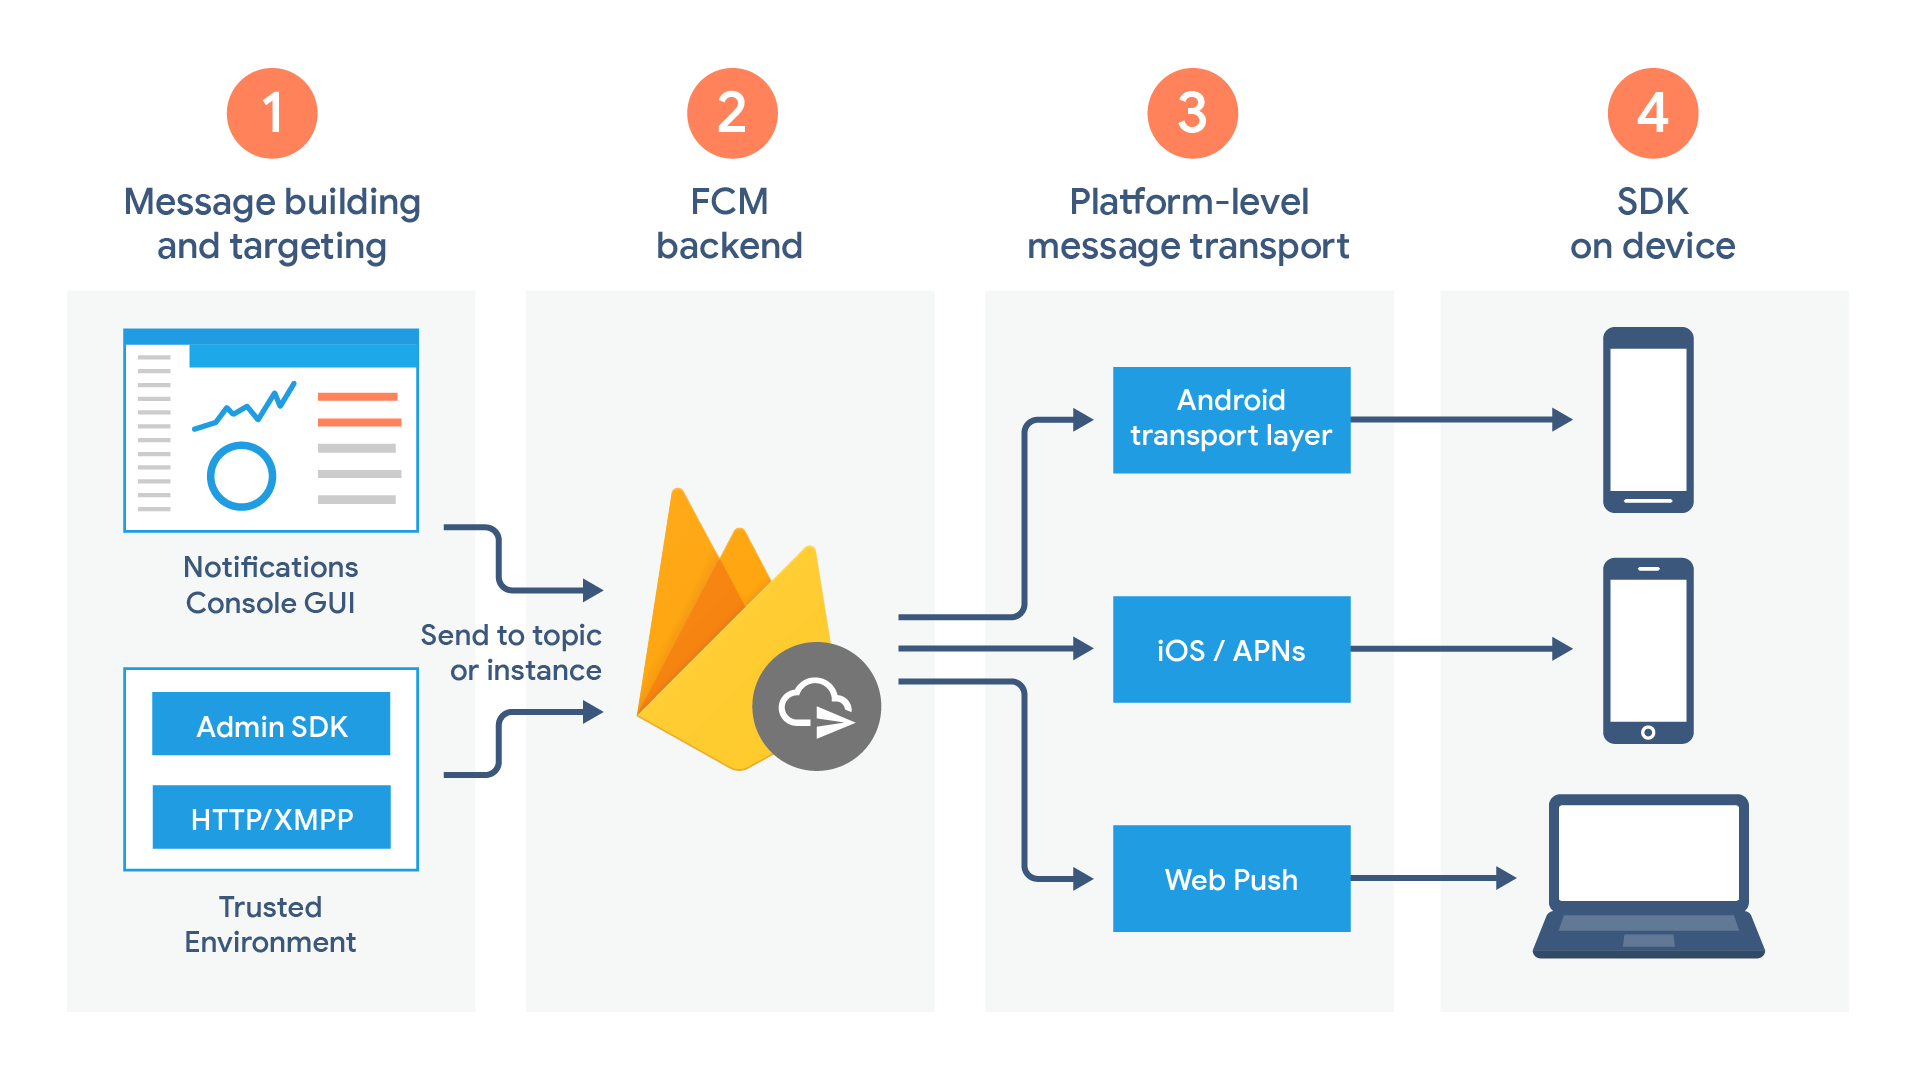
\includegraphics[scale=0.23]{Theoretische_Grundlagen/images/firebase_cloudmessaging_architecture.png}
	\end{center}
	\caption{Firebase Cloud Messaging Architektur}
	\label{fig:cloudmessaging_architecture}
\end{figure}

\subsubsection{Google AdMob}
Google AdMob bietet eine einfache Art, gezielte Werbung innerhalb der Anwendung zu schalten und somit die Anwendung zu monetarisieren.
Zusätzlich bietet das Tool in Kombination mit Google Analytics\footnote{Ein freies Analysetool, welches über alle Tools hinweg Ereignisse sammelt und diese Werte direkt graphisch darstellt. Da es für die Implementierung nicht weiter relevant ist, wird es nicht detaillierter besprochen. Zusätzliche Informationen unter \href{https://firebase.google.com/docs/analytics}{firebase.google.com}.} zusätzliche Anwendungsdaten und Analysefähigkeiten.\\
Werbung lässt sich in unterschiedlicher Weise anzeigen (siehe Abbildung \ref{fig:firebase_admob})und lässt sich reibungslos in UI Komponenten integrieren. 
Verschiedene Features sind hier jedoch plattformabhängig. 
Auf der Android Plattform ist es für Nutzer möglich, beworbene Produkte direkt aus der Anwendung heraus zu kaufen.\\
Ein weiteres Werbetool \textit{Google Mobile Ads SDK} ist eine alleinstehende SDK, hingegen Google AdMob bietet einfache Integration in Firebase und weitere Tools.\cite{firebase2021}

\begin{figure}[htb]
	\begin{center}
		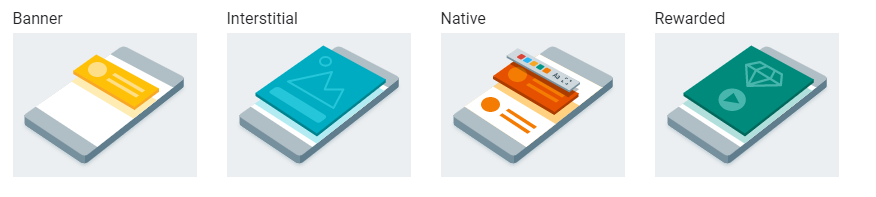
\includegraphics[scale=0.55]{Theoretische_Grundlagen/images/firebase_admob_ads.PNG}
	\end{center}
	\caption{Google AdMob Anzeigemöglichkeiten}
	\label{fig:firebase_admob}
\end{figure}




































